\documentclass[11pt, a4paper]{article}
\usepackage[utf8]{inputenc}
\usepackage[T1]{fontenc}
\usepackage[margin=1in]{geometry}
\usepackage{microtype}
\usepackage{graphicx}
\usepackage{caption}
\usepackage{subcaption}
\usepackage{booktabs}
\usepackage{amsmath,amssymb}
% \usepackage{siunitx}
\usepackage[authoryear,round]{natbib}\usepackage{setspace}
\usepackage{lineno}
\usepackage{xcolor}
\usepackage[hidelinks]{hyperref}
\usepackage{multirow}
\usepackage{float}
\usepackage{xr} % for referencing between different .tex files
% \usepackage{citation-style-language}
% \cslsetup{style = palaeontology}
% \addbibresource{references.bib}
\setcitestyle{aysep={}}  % Removes comma between author and year. need to reformat to match palaeontology journal style?
\newcommand{\ASE}{Ancestral state estimation }
\newcommand{\ase}{ancestral state estimation }
\externaldocument{supplementary}
% Line spacing and numbering for review
\doublespacing
\linenumbers

\title{Incorporating ancestral state estimation uncertainty can improve disparity analyses}

\author{Caleb Scutt\textsuperscript{1,2*}, Natalie Cooper\textsuperscript{2}, Gavin H. Thomas\textsuperscript{1}, Thomas Guillerme\textsuperscript{1}}

\date{}

\begin{document}

\maketitle

\begin{center}
\small
\textsuperscript{1}School of Biosciences, University of Sheffield, Sheffield, UK\\
\textsuperscript{2}Science Group, Natural History Museum, London, UK\\[12pt]
*Corresponding author: cnscutt1@sheffield.ac.uk 
\end{center}


\begin{abstract}
\noindent
Morphological trait datasets and phylogenies are routinely paired to investigate macroevolutionary patterns during disparity analyses.
However, incomplete fossil sampling can distort disparity estimates, obscuring true evolutionary signals.
Ancestral state estimation can be used for both continuous and discrete traits to extend these analyses beyond incomplete fossil data and generate a more complete trait space.
However, when ancestral state estimation occurs in the disparity pipeline, and the inevitable uncertainty in these estimates, complicate their integration.
Determining the most robust workflow for integrating ancestral state estimation in disparity analyses remains a critical methodological challenge.
Using simulations to attain a ground-truth disparity value, we evaluated different approaches to performing ancestral state estimation and incorporating uncertainty across varying continuous and discrete trait models, fossil sampling densities and disparity metrics.
Ancestral state estimation generally improved recovery of true disparity relative to tip-only analyses, though the optimal approach depended on the interaction between trait model and fossil sampling density.
For continuous traits, probabilistic approaches were most accurate, but were sensitive to model misspecification under low fossil sampling density.
For discrete traits, pre-ordination methods were most reliable and probabilistic approaches outperformed point estimates under low sampling, while point estimates became increasingly accurate as sampling density increased.
Fossil sampling density was a stronger predictor of disparity accuracy than estimation method choice, underscoring that methodologies are only as powerful as the data provided.
Our findings offer a practical decision framework for selecting the most appropriate workflow given the sampling density and trait characteristics of a dataset.

\end{abstract}

\noindent\textbf{Keywords:} ancestral state estimation; disparity; fossils; simulation; uncertainty; macroevolution

\section{Introduction}

Morphological diversity, hereafter termed disparity, is widely used for investigating macroevolutionary dynamics \citep{foote1997evolution,wills2001morphological,guillerme2020disparities}.
Disparity can be described as the distribution or spread of taxa within a multidimensional trait space defined by morphological similarity \citep{erwin_disparity_2007} and can be quantified using both continuous \citep{garcia2017phenotypic,gray2019exceptional, friedman2020body} and discrete characters \citep{foote1994morphological, lloyd2016estimating}.
Morphological trait datasets are routinely integrated with phylogenies when examining disparity across clades or time.
These analyses can be used to investigate selectivity across mass extinctions \citep{bapst2012graptoloid,cole2021selectivity, liu2024heterogeneous}, reveal patterns in morphological convergence \citep{muschick2012convergent,stayton2015definition,stayton2024does} or characterise the tempo and mode of morphological diversification during adaptive radiations \citep{harmon2003tempo,mahler2010adaptive, hughes2013clades}.
However, such analyses are inevitably limited by the incompleteness of the fossil record; only a biased subset of past diversity is preserved, leaving phylogenetically-implied ghost taxa and obscuring large portions of a clade's evolutionary history \citep{norell1993tree, wagner1995stratigraphic,flannery2019does,smith2021phylogenetic}.
These missing data can result in both under- and over-estimations of disparity \citep{mitchell2015extant,smith2023fossilization}.

One way in which unsampled lineages can be accounted for is through the use of ancestral state estimation.
\ASE is the method of estimating trait value(s) in a set of common ancestors, i.e., nodes on a phylogenetic tree, given a set of tip data \citep{schluter1997likelihood,cunningham1998reconstructing,revell2025ancestral}.
% This involves the unification of our observed trait data with a phylogeny, enabling a switch from simply observing a pattern (points in trait space) to inferring a process through time. 
% \ASE has been used extensively across macroevolutionary studies for inferring the likely character state at each node on a phylogeny for continuous or discrete traits of interest \citep{meloro2012tooth, esquerre2019mountains, morris2019heterochronic}.
These estimated states can be combined with the observed tip data to generate a more complete trait space, filling the gaps left by an incomplete fossil record and, in theory, improving our ability to recover the `true disparity' of a group \citep{sidlauskas2008continuous,brusatte2011phylogenetic,lloyd2018journeys}.
True disparity in this context can be defined as the total trait space occupied by all lineages throughout a clade's history, measured by either volume or density \citep{guillerme2020shifting}.
Crucially, the inclusion of ancestral states allows disparity through time analyses to be explored with higher temporal resolution \citep{brusatte2011phylogenetic, halliday2016eutherian, guillerme2018disprity}.

Despite the aforementioned advantages, the use of \ase within disparity analyses has often been neglected.
The hesitancy to incorporate \ase has likely stemmed from the notion that estimates are inherently uncertain; root-ward estimates in particular are often associated with large confidence intervals or inconclusive scaled likelihoods \citep{schluter1997likelihood, losos1999uncertainty,gascuel2014predicting}.
Despite the encouragement to propagate uncertainty during comparative analyses \citep{silvestro2015measurement,boyko2024dentist}, ancestral state estimations are generally treated as point estimates during disparity analyses, because there is little guidance on how to correctly treat \ase uncertainty downstream when constructing the trait space. %@@@keating line 63
These point estimates are typically the maximum likelihood estimates for continuous characters or collapsed states returned from arbitrary thresholds for discrete characters \citep{smith2022evolution,casali2023morphological, li2026morphological}.
By ignoring ancestral state estimation uncertainty, point estimates can lead to overconfidence in results and incorrect inferences in downstream analyses, all while obscuring potentially accurate signals \citep{ackerly2006niche,vanderpoorten2006mapping}.

Another key issue with \ase is its sensitivity to model misspecification.
Likelihood-based approaches to \ase require both a tree topology and a specified model of character evolution.
Continuous character estimations are typically modelled under Brownian motion (BM; but see \citealp{elliot2014inferring, castiglione2020ancestral, meade2022ancestral}), which describes a directionless, stochastic process where the trait divergence between related taxa is proportional to their shared evolutionary history and the rate of evolution \citep{felsenstein1985phylogenies,schluter1997likelihood,omeara2006testing}.
However, deviations from BM in the trait data, such as directional trends or stabilising selection, inevitably returns biased estimates \citep{webster2002testing, finarelli2006ancestral, albert2009fossils,finarelli2013potential}. 
% For example, both \cite{webster2002testing} and \cite{finarelli2006ancestral} were unable to recover accurate ancestral estimates of body size in planktonic Foraminifera and mammals, respectively, due to a trend of increase through time.
Model-related issues can also arise for discrete traits, which are estimated using M\textit{k} \citep{lewis2001likelihood,pagel1994detecting,pagel1999maximum} or SSE models \citep{ng2014traits, holland2020accuracy}. %@@@keating line 81
Estimation accuracy of discrete states appears prone to model over-parameterisation and sensitive to fast transition rates \citep{mooers1999reconstructing, keating2023best}.
Furthermore, discrete \ase faces a paradoxical trade-off where a slow rate of evolution allows for an accurate estimation of the root state, but provides little information for calculating transition rates \citep{gascuel2020darwinian}.
Similarly, the opposite is true whereby fast rates allow for an accurate estimation of transition rates, but uncertainty in the root state estimation.%@@@keating line 83

Given that uncertainty is often high in ancestral state estimation, how then can estimates be improved?
\ASE is statistically inconsistent, meaning that even if the sample size of extant tips were infinite, estimates are not expected to converge on the true value \citep{ane2008analysis}.
The inclusion of fossils can improve estimations by breaking long branch lengths, reducing distance between tips and internal nodes \citep{finarelli2006ancestral,finarelli2013potential,joy2016ancestral, goswami2025morphological}.
Numerous simulation and empirical based studies have shown that ancestral state estimations based on extant-taxa only are biased \citep{webster2002testing,finarelli2006ancestral,albert2009fossils,betancur2015fossil,royer2016comparison,monson2022keeping,wisniewski2022extant,keating2023best}, though this bias can be driven by model misspecification rather than missing data alone \citep{goldberg2008phylogenetic, puttick2015fossils}.
Similar biases have been observed in extant-only disparity analyses \citep{mitchell2015extant}. 
Despite this, many studies are forced to use extant-only trees for both ancestral state estimation \citep{jetz2018interplay, amador2021evolution} and disparity \citep{harmon2010early,baker2015adaptive,smith2022evolution} due to a lack of viable fossil data.

Numerous studies have assessed the raw estimation error of \ase approaches under different models of evolution, methods of estimation and fossil sampling density \citep{elliot2014inferring,royer2016comparison, reyes2018testing, holland2020accuracy,keating2023best,boyko2026resolving}.
However, how trait estimation accuracy is propagated into the recovery of an accurate trait space is less understood, despite the continued use of \ase in disparity analyses.
One methodological debate concerns whether \ase should be conducted before or after trait space ordination.
Previous work has found that carrying out \ase on the axes of an ordination matrix rather than raw characters can distort the distribution of points in a trait space markedly, introducing unwanted phylogenetic signal and low levels of convergence \citep{lloyd2018journeys}.
However, this study was restricted to a single empirical dataset and discrete traits.
Thus, we lack a comprehensive understanding of how estimation approaches, trait data and fossil sampling density interact to affect our ability to recover accurate patterns in trait space and therefore disparity.

Here we evaluate the ability of different \ase approaches to recover true disparity values across different evolutionary models and fossil sampling densities using a simulation framework.
Simulations offer a robust approach for benchmarking methodologies because a ground-truth dataset can be generated, so trait values and the resulting disparity value are all known \textit{a priori} \citep{lotterhos2022simulation}.
Different methodological choices and estimation scenarios can then be evaluated against the true disparity value.
Specifically, we directly compare pre- versus post-ordination ancestral state estimation approaches, as well as point-estimate versus probabilistic treatments of uncertainty.
We also investigate how estimation error varies under different models of continuous (Brownian motion with and without trend and Ornstein-Uhlenbeck) and discrete traits (varying transition rates), fossil sampling densities (100\%, 50\%, 15\%, 5\% and 0\% of extinct lineages) and disparity metrics examining size and density.
This integrative approach provides a comprehensive evaluation of when \ase improves disparity estimation, when it introduces bias, and how uncertainty should be treated when working with an incomplete fossil record.

\section{Materials and Methods}

\subsection{Simulation Framework}
\subsubsection{Phylogenies}
All simulations were generated using \texttt{treats} in R v.4.4.1 \citep{guillerme2024treats,Rlanguage}.
We simulated birth-death trees with the speciation ($\lambda$) parameter set to 1.0, and extinction ($\mu$) set to 0.9 (\autoref{fig:pipeline} Step 1).
% Fixing $\lambda = 1.0$ provides a convenient relative timescale, because only the ratio of extinction to speciation affects the shape and balance of simulated trees.
This fraction of extinction ($\mu = 0.9$) produces trees that match our expectation of substantial extinct diversity based on the fossil record \citep{scholl2016diversification,pires2018diversification, henao2019macroevolutionary,morlon2024phylogenetic}.
% These parameters correspond to a high turnover regime, consistent with the upper-empirical estimates from diversification studies of animal groups \citep{scholl2016diversification,pires2018diversification, henao2019macroevolutionary,morlon2024phylogenetic}. 
% This fraction of extinction ($\mu = 0.9$) produces trees that match our expectation of substantial extinct diversity based on the fossil record.
We generated three sets of 100 birth-death trees with these parameters until the simulations reached 50, 100 or 150 extant taxa, with maximum tree size of 500, 1000 and 1500 tips, respectively (\autoref{fig:tree sizes}).
The randomness of the birth-death model meant some simulated trees contained only extinct taxa, so we re-ran each individual simulation until we obtained the desired number of extant taxa.
This meant that although the parameters were set to $\lambda = 1$ and $\mu = 0.9$, the effective parameters slightly deviated from these input values (\autoref{fig:net div overall trees}).
Mean net diversification across all simulated trees was $0.30\pm0.09$.
Constant birth death parameters meant that the simulated trees were highly symmetrical (\autoref{fig:main trees colless dist}).
Given that empirical palaeontological phylogenies tend to be imbalanced \citep{harcourt2001imbalance}, we also simulated 100 birth-death trees with high asymmetry and ran the same pipeline (\autoref{fig:assymetrical trees colless dist}).
Trees were pruned to extract the crown clade of the tree for downstream analyses.
This ensured that all downsampled trees shared an identical root node and tree height with the original tree simulation.
Therefore, any tip included in the analyses was a descendant of the most basal node considered, i.e., the MRCA of extant tips, ensuring that all ordinations and disparity values were calculated within a consistent clade. %@@@keating line 147


\begin{figure}[H]
\centering
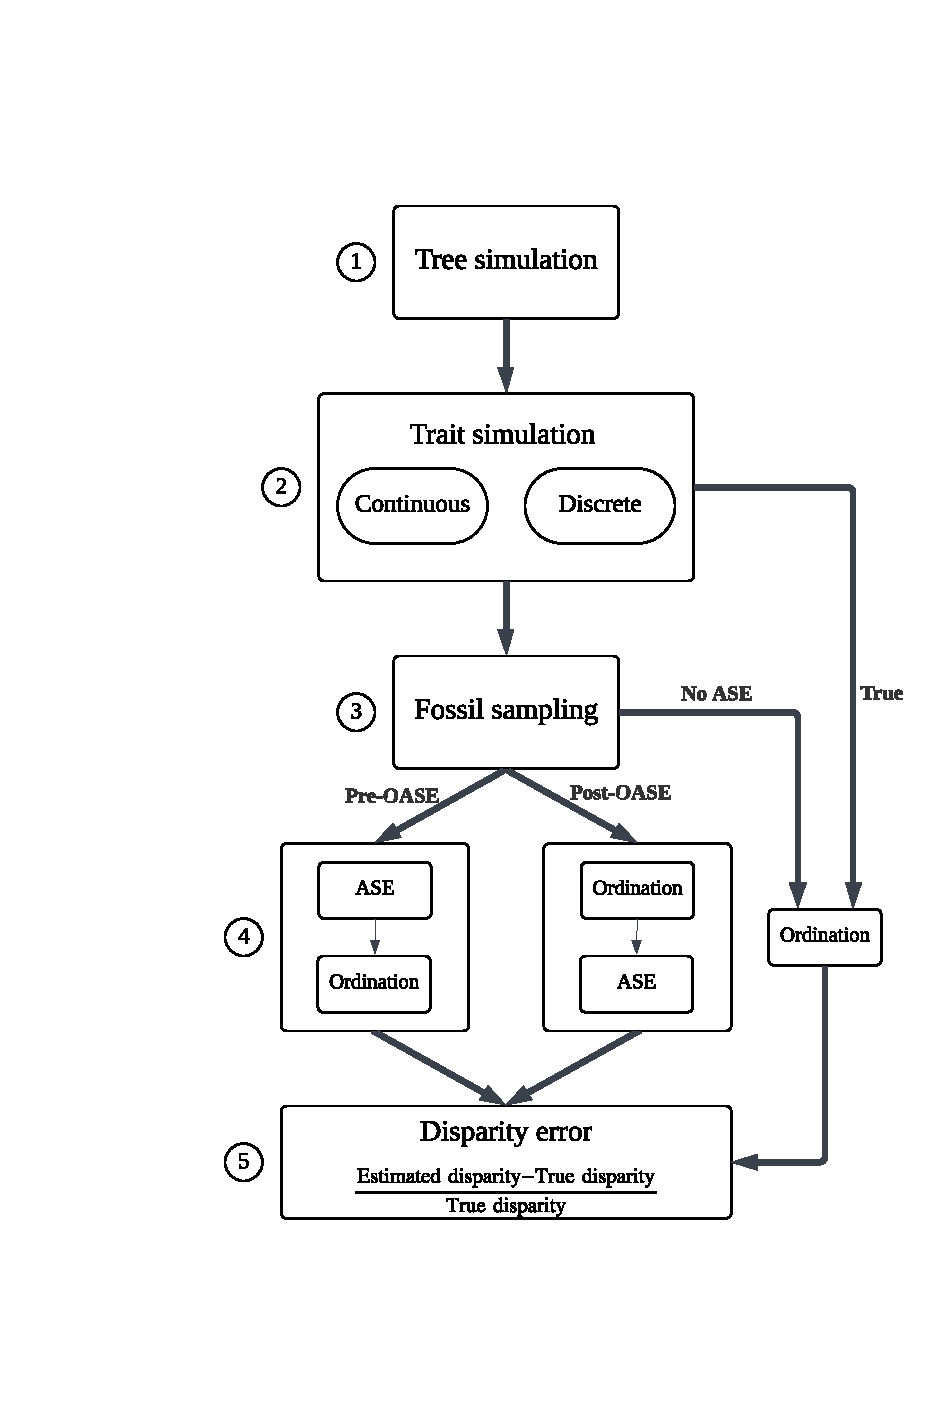
\includegraphics[width=0.8\textwidth]{figures/ACEDisparity_pipeline.pdf}
\caption{Overall simulation pipeline, highlighting the five different estimation routes (pre-ordination point, pre-ordination distribution, post-ordination point, post-ordination distribution and no ancestral state estimation) as well as the true route, from which ground-truth disparity value is calculated from the untreated simulation.}
\label{fig:pipeline}
\end{figure}


\subsubsection{Trait simulations} \label{trait simulation}
For each phylogeny, we simulated continuous and discrete trait data separately (\autoref{fig:pipeline} step 2). 
Continuous trait data were simulated under variations of Brownian motion (BM) and Ornstein-Uhlenbeck (OU) models (\autoref{tab:models}).
We simulated BM with variance = 0.25.
We also simulated BM with a trend parameter of 0.3, where the ancestral trait value increased incrementally proportional to branch length.
OU trait data were simulated with the $\alpha$ parameter set based on phylogenetic half-life to account for differing tree heights across simulations \citep{gearty2024impact}.

\begin{equation}
\alpha=\dfrac{\ln(2)}{\text{tree height $\times$ 0.25}}
\end{equation} 

\noindent We simulated 20 independent characters for each model (BM, BM + trend and OU) across each phylogeny.

Discrete trait evolution was simulated using a discrete-time Markov process, where the probability of state transition along each branch was proportional to the product of the transition probability and branch length.
We simulated discrete traits across three rate categories, representing fast (0.9), medium (0.1) and slow (0.01) transition rates (\autoref{tab:models}).
These rates were assigned by generating equal-rates (ER) transition probability matrices.
For each category, 85 binary characters and 15 three-state characters were simulated, following a typical scoring ratio found in empirical data \citep{guillerme2016effects, casali2023morphological}.

\begin{table}[H]
\centering
\caption{Simulation models and parameters used for phylogeny generation and trait evolution. For continuous characters, the root state was always set to 0. $\lambda$ = speciation; $\mu$ = extinction; $P_{ij}$ = transition rate; $\sigma^2$ = evolutionary variance; $\theta$ = optimum, $\alpha$ = rate of adaptation toward the optimum.}
\label{tab:models}
\begin{tabular}{|c|c|c|}
\hline
\textbf{Data generation} & \textbf{Model} & \textbf{Parameters} \\
\hline
\textbf{Phylogeny} & Birth-death & $\lambda=1.0,\ \mu=0.9$, extant tips = $50, 100, 150$ \\
\hline
\multirow{3}{*}{\textbf{Continuous traits}} & $BM$ & $\sigma^2=0.25$ \\
\cline{2-3}
 & $BM + trend$ & $\sigma^2=0.25,\ \text{trend}=0.3$ \\
\cline{2-3}
 & $OU$ & $\sigma^2=0.25,\ \theta = 0, \alpha=\dfrac{\ln(2)}{\text{tree height} \times 0.25}$ \\
\hline
\multirow{3}{*}{\textbf{Discrete traits}} & $Fast$ & $P_{ij}=0.9$ \\
\cline{2-3}
 & $Medium$ & $P_{ij}=0.1$ \\
\cline{2-3}
 & $Slow$ & $P_{ij}=0.01$ \\
\hline
\end{tabular}
\end{table}


\subsection{Fossil sampling simulation}
To explore the interaction of fossil sampling with estimation method on the disparity accuracy, we simulated fossil sampling in two ways.
The first way, labelled 'tips-only', is that extinct tips were either retained (`fossilised') or pruned using a Bernoulli sampling method at five different probabilities: 0\%, 5\%, 15\%, 50\% and 100\% (\autoref{fig:pipeline}: Step 3).
This method meant each extinct tip had an equal probability of being `fossilised' at each sampling level, irrespective of the total tree size.

To test whether our fossil sampling scheme was biased by only sampling tips, we also used the same Bernoulli sampling method but allowed nodes to be sampled as well as tips, labelled 'tips+nodes'. %@@@wagner line 175
Sampled nodes were attached to the tree as tips using the \texttt{phytools::bind.tip} function \citep{revell2012phytools} with a non-zero branch length.
The corresponding trait matrices were subset to match the tips remaining in each down-sampled tree, with all extant taxa sampled across all fossil sampling densities.
From herein, these resulting downsampled trees and matrices are referred to as sampled-taxa.

\subsection{Ancestral state estimation (ASE)} 
We estimated the ancestral states of the sampled-taxa using \texttt{dispRity::multi.ace} \citep{guillerme2018disprity}, which is a wrapper for \texttt{ape::ace} \citep{paradis2019ape}.
We used four combinations of two approaches to ancestral state estimation to evaluate each method's accuracy in recovering true disparity values (\autoref{fig:pipeline}: Step 4).
These were then compared to a null of bypassing ancestral state estimation whereby only sampled-taxa were used to generate trait spaces.

\subsubsection{Pre-ordination estimation} \label{pre-ord}
Ancestral state estimation of trait data can be carried out at two points either side of the ordination step in the pipeline (\autoref{fig:pipeline}: Step 4; \citealp{lloyd2018journeys}).
Pre-ordination \ase estimation involves the estimation of the raw trait values for each node. We performed pre-ordination estimation of continuous characters under a BM model, where ancestral state values lie within a multivariate normal distribution that is estimated given the observed tip data and the shared evolutionary history among taxa \citep{schluter1997likelihood,rohlf2001comparative}.
The width of the estimated confidence interval returned reflects the uncertainty in continuous ancestral estimates, typically increasing with node depth and decreasing with the number of informative descendant lineages.

Pre-ordination estimation of discrete characters involves estimating the marginal likelihoods for each discrete state at each node, based on a maximum likelihood derived estimate of the M\textit{k} transition matrix and the tree topology given \citep{pagel1999maximum,yang2006computational}.
Given that the transition rates were set \textit{a priori} during simulations, the equal-rates (ER) model was used to avoid model misspecification as a confounding factor on estimation accuracy \citep{keating2023best}.
%CS: could do an analysis where ARD model is used to see if results change with model mispecification (Russell mentioned this)? TG: this is also a very good point like the one for the different fossilisation biases but I think we should keep it to what it is for now and then add/remove depending on the reviews.

We constructed trait spaces for disparity estimation by ordinating the matrices of combined sampled-taxa and ancestral node states.
Continuous data were ordinated using principal components analysis (PCA; \texttt{stats::prcomp}). 
Because PCA requires raw continuous data to calculate covariance, discrete characters were instead converted to distance matrices using the Maximum Observed Rescaled Distance metric (MORD) \citep{lloyd2016estimating} and ordinated using principal coordinates analyses (PCoA; \texttt{stats::cmdscale}) using the Cailliez correction to deal with negative eigenvalues \citep{cailliez1983analytical}.

\subsubsection{Post-ordination estimation} \label{post-ord}
Post-ordination estimation calculates the continuous PC scores across each axis of an ordination matrix for each ancestral node.
For post-ordination ancestral state estimation, PCA and PCoA were applied prior to ancestral state estimation to the down-sampled continuous and discrete character matrices, respectively, to generate a set of sampled-taxa trait spaces.
Ancestral node states were then estimated under a Brownian motion model across all PC axes, as detailed in \autoref{pre-ord}.


\subsubsection{Uncertainty treatment} \label{uncertainty}
For each estimation method, we also compared point estimate and probabilistic approaches.
The point estimate approach returned a fixed single value for each estimate.
For continuous characters, the point estimate returned by \texttt{ape::ace} is the single maximum likelihood estimate of the ancestral state.
For discrete characters, we used a strict majority rule where the state with the highest scaled likelihood was selected at each node for each character.
When state likelihoods were tied one state was selected at random.
% We also used a relative majority rule, where any state at a scaled likelihood greater than the maximum observed scaled likelihood minus the inverse number of possible states was collapsed, otherwise states were left as uncertain (supplementary).

The probabilistic approach differed in that uncertainty was explicitly accounted for by sampling multiple estimates rather than a single point.
For continuous characters, we sampled each state across 100 matrices, with each estimate value lying within a normal distribution centered on the single point estimate and spread across the 95\% confidence interval.
Each discrete character state at each node was also sampled across 100 matrices according to their scaled likelihoods.
In a scenario where there is uncertainty in a binary character at a specific node, e.g., 0.55 for state 0 and 0.45 for state 1, this distribution approach results in a 55\% probability of sampling state 0 in each matrix for the respective node (and 45\% chance of sampling state 1).
Both procedures were implemented using the \texttt{sample = 100} argument in \texttt{dispRity::multi.ace} \citep{guillerme2018disprity}.


\subsection{Disparity analyses}
Our aim for this study was to understand how well ancestral state estimation can recover true properties of size and density in trait space occupancy, measured by disparity metrics \citep{guillerme2020shifting}.
% Since we were assessing overall disparity, position was not a metric that can be discerned due to the centring of ordinated matrices. TG: this sentence is probably not necessary. But might bring it back if a reviewer asks for why no position?
Size-based metrics describe the volume of trait space the clade occupies \citep{guillerme2020shifting}.
To examine how well the size of the trait space was recovered, we calculated the sum of quantiles.
The sum of quantiles measures the 95\% interpercentile range on each PC axis and then sums these ranges.
This metric has similar properties to the often used sum of ranges metric by describing the total trait space exploited \citep{foote1992rarefaction}, but with less sensitivity to outliers and sample size.
For density, we calculated the sum of variances \citep{ciampaglio2001detecting,wills2001morphological} and the mean pairwise distance \citep{ciampaglio2001detecting}. 
To quantify methodological performance, we calculated these disparity metrics for the ground-truth simulated trait spaces, the sampled-taxa only trait spaces, and the spaces generated by each \ase approach so that relative disparity errors could be calculated (\autoref{fig:pipeline} step 5).
Given that the dimensionality of discrete trait spaces varied across fossil sampling densities within the same replicate, we also ran analyses where dimensionality was constrained to the minimum number of axes reached across all fossil sampling levels, i.e., for the 50 living-taxa trees, this was 48 dimensions.

\begin{equation}
\text{Relative disparity error} = \frac{\text{Estimated disparity} - \text{True disparity}}{\text{True disparity}}
\end{equation}

\subsection{Statistical tests}
The relative disparity errors were converted to absolute relative errors to measure the magnitude of deviation from the true disparity, regardless of direction.
Due to the zero-inflated and right-skewed nature of the error distribution, we applied a log-transformation.
Consequently, the more negative the log-error, the more accurate (closer to $log(0)$) the original estimation.
Given the imbalance in sample sizes between the different uncertainty treatments (i.e., distribution approaches returned 100 disparity values per estimate, whereas point estimates returned one), we aggregated the distribution outputs by taking the median prior to analyses.
We also performed analyses where the distribution was retained, but each individual point returned by distributions was weighted 1/100th of the single point estimate.
% Results were consistent between both approaches (\autoref{fig:weighted LMM continuous heatmap}; \autoref{fig:weighted LMM discrete heatmap}).

We investigated the drivers of disparity estimation accuracy with linear-mixed models (LMM) using the \texttt{lme4} R package (\citealp{bates2015fitting}; \autoref{fig:cont lmm diagnostic aggregated}, \ref{fig:discrete lmm diagnostic aggregated})
The log-transformed relative error was treated as the response variable. 
Based on our experimental design, we fitted a four-way interaction between the estimation method, model of evolution, fossil sampling density and disparity metric.
We also included tree size as a further non-interactive fixed effect.
To account for the variation with each simulation run, each tree replicate was included as a random intercept.
We carried out \textit{post-hoc} pairwise comparisons using estimated marginal means, adjusted using Tukey's honestly significant difference (HSD) \citep{lenth2025emmeans}.


\section{Results}
The results reported herein are from the aggregated linear mixed-effects models (LMMs) from the tips-only fossil sampling simulation analysis retaining all PC axes in trait space.
Results from the weighted distribution point LMMs were consistent with these findings (\autoref{fig:weighted LMM continuous heatmap}, \ref{fig:weighted LMM discrete heatmap}).
\subsection{Continuous traits}
\subsubsection{Estimation methods}
For continuous characters, the estimation method had a significant effect on disparity accuracy ($F_{4,66976} = 358, ~ p < .001$; \autoref{fig:continuous boxplot}).
Notably, using ancestral state estimation methods improved estimates of disparity compared to excluding ancestral states when averaged over all scenarios.
\textit{Post-hoc} pairwise comparisons of estimated marginal means (EMM) revealed both pre- and post-ordination distributions of ancestral state estimations returned the lowest log disparity errors (Table S1). 
In contrast, point estimates performed worse overall than bypassing ancestral state estimation altogether.

\begin{figure}[H]
\centering
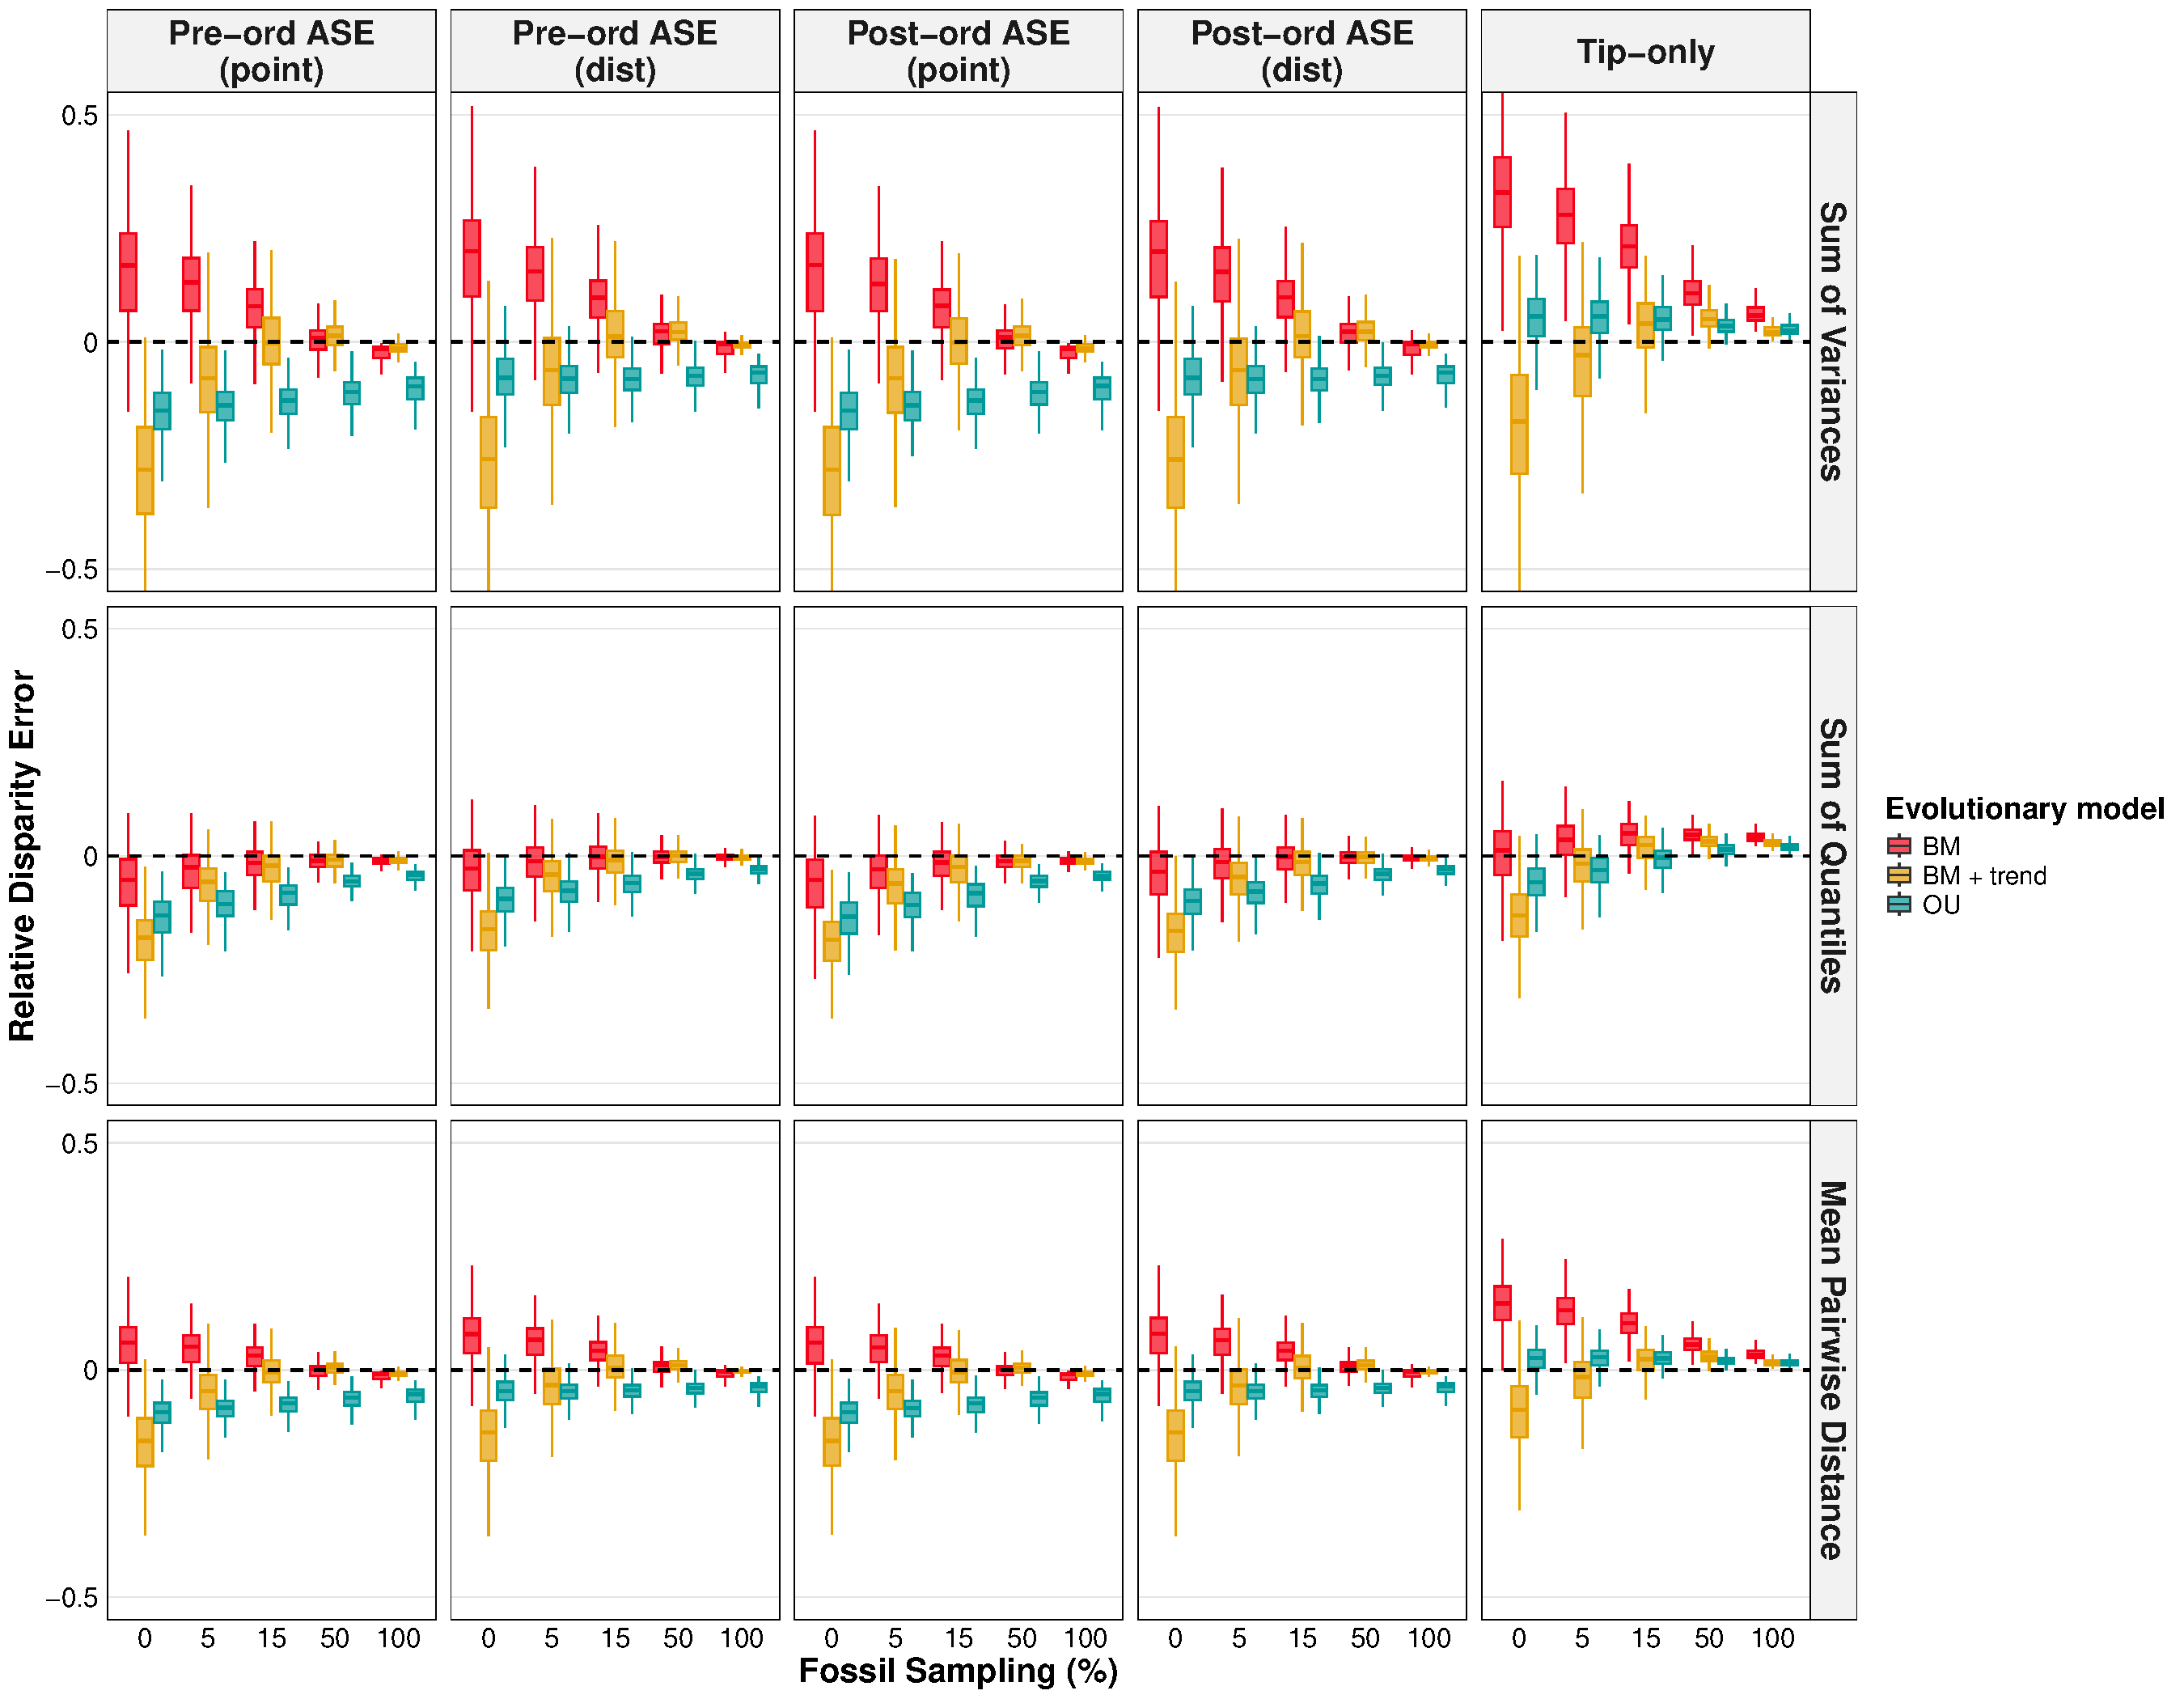
\includegraphics[width=1\textwidth]{figures/continuous_boxplot.pdf}
\caption{Relative disparity error returned from pre-ordination point ancestral state estimation (ASE), pre-ordination distribution ASE, post-ordination point ASE, post-ordination distribution ASE and no ASE. These disparity errors were calculated across three evolutionary models (Brownian motion (BM), BM + trend and OU), five simulated fossil sampling densities (100\%, 50\%, 15\%, 5\% and 0\%) and three disparity metrics (Sum of variances, sum of quantiles and mean pairwise distance). Values closest to 0 (dotted horizontal line) were most accurate; negative errors are under-estimates and positive are over-estimates.} 
\label{fig:continuous boxplot} 
\end{figure}


\subsubsection{Interaction effects}
The pattern that \ase methods improved estimates of disparity was context-specific (\autoref{fig:continuous heatmap}).
Fossil sampling was the strongest driver of recovery of an accurate disparity value for continuous traits ($F_{4,66976} = 9169, ~ p < .001$), as each increase in fossil sampling density resulted in a significant reduction in disparity error.
Similarly, the evolutionary model ($F_{2,66976} = 2956, p < .001$) and disparity metric ($F_{2,66976} = 5028,~ p < .001$) were also strong drivers of variation in error.
Specifically, disparity outputted from the BM models and sum of quantiles metric were associated with better disparity estimates, whereas the OU model and sum of variances were the least accurate.
Tree size had a minor effect in comparison ($F = 43_{2,297},~ p < .001$).
The three-way interaction between estimation method, fossil sampling and evolutionary model was significant ($F_{32,66976} = 60,~ p < .001$) and the \textit{post-hoc} EMM can be used to identify the optimal method for models at each fossil sampling density (Table S2).
For Brownian motion (BM) at 100\% fossil sampling, the distribution estimations were most accurate. 
At 50\% and below, methods of \ase generally performed equally well and significantly better than excluding ancestral states.
Under BM + trend, a similar pattern was followed at high fossil sampling densities, yet when fossil sampling dropped below 15\% methods of \ase performed worse than excluding ancestral states. 
In contrast, under an OU model the exclusion of ancestral states was the best approach across all fossil sampling densities.
While the disparity metric had a large effect on the overall estimation accuracy, it was a relatively lower driver of variation regarding its interaction with the estimation method ($F_{8,66976} = 7,~ p < .001$).
Therefore, while estimation accuracy differed between metrics, the hierarchy between optimal methods was generally consistent across metrics.

\subsubsection{Sensitivity tests} 
These findings were largely congruent under the alternative tips+nodes fossil sampling scheme, albeit we found that excluding ancestral states was marginally better performing when using the sum of quantiles metric across all models (\autoref{fig:Continuous nodes tips boxplot}).

\begin{figure}[H]
\centering
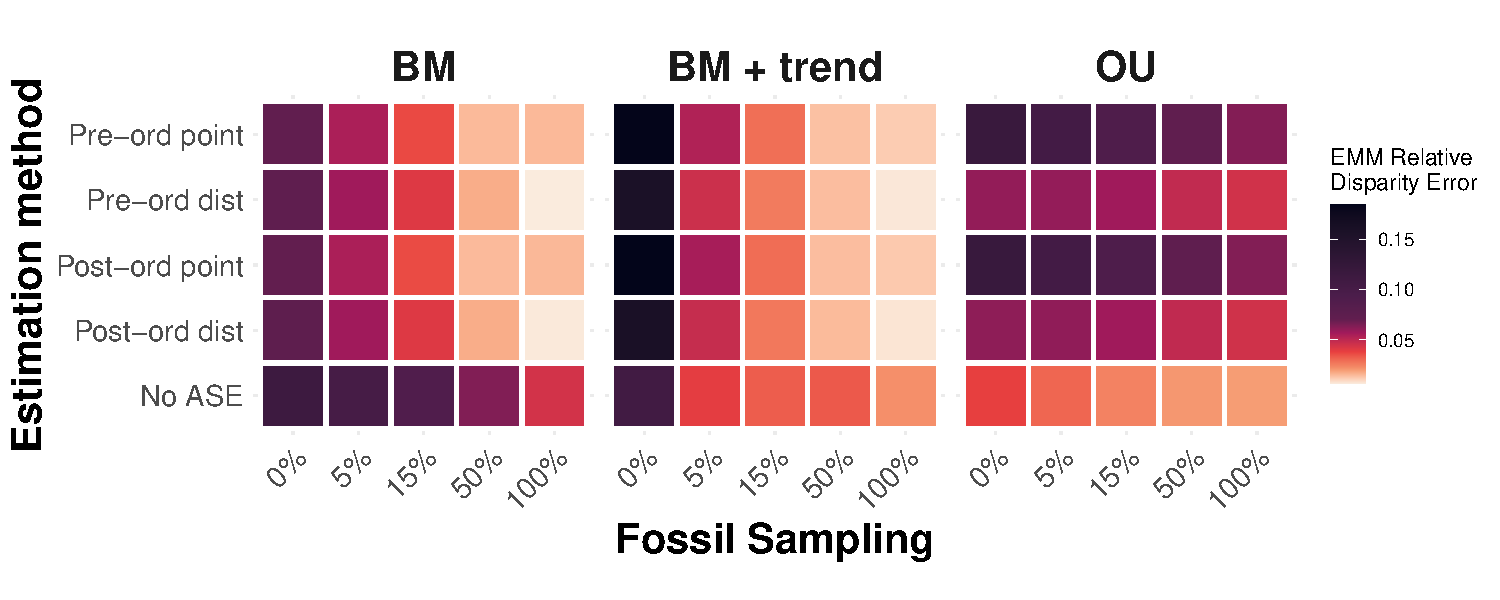
\includegraphics[width=1\textwidth]{figures/cont_heatmap.pdf}
\caption{Heatmap presenting the continuous estimated marginal mean (EMM) relative disparity errors for every combination of estimation method, evolutionary model and simulated fossil sampling density. EMM were calculated from a linear mixed model with a three-way interaction term, averaged across disparity metrics.} 
\label{fig:continuous heatmap} 
\end{figure}

\subsection{Discrete traits}
\subsubsection{Estimation methods} 
For discrete characters, the estimation method also had a significant effect on disparity accuracy ($F_{4,66976} = 10767,~ p < .001$; \autoref{fig:discrete raw boxplot}).
Similar to continuous traits, methods of ancestral state estimation consistently improved disparity estimates compared to excluding ancestral states. 
However, the optimal type of estimation differed. 
\textit{Post-hoc} pairwise comparisons of EMM revealed that pre-ordination point estimates returned the lowest log disparity errors overall. 
In contrast to continuous traits, distribution methods generally performed worse than pre-ordination point estimates on average, but post-ordination point estimates performed worse than excluding ancestral states (Table S3).

\begin{figure}[H]
\centering
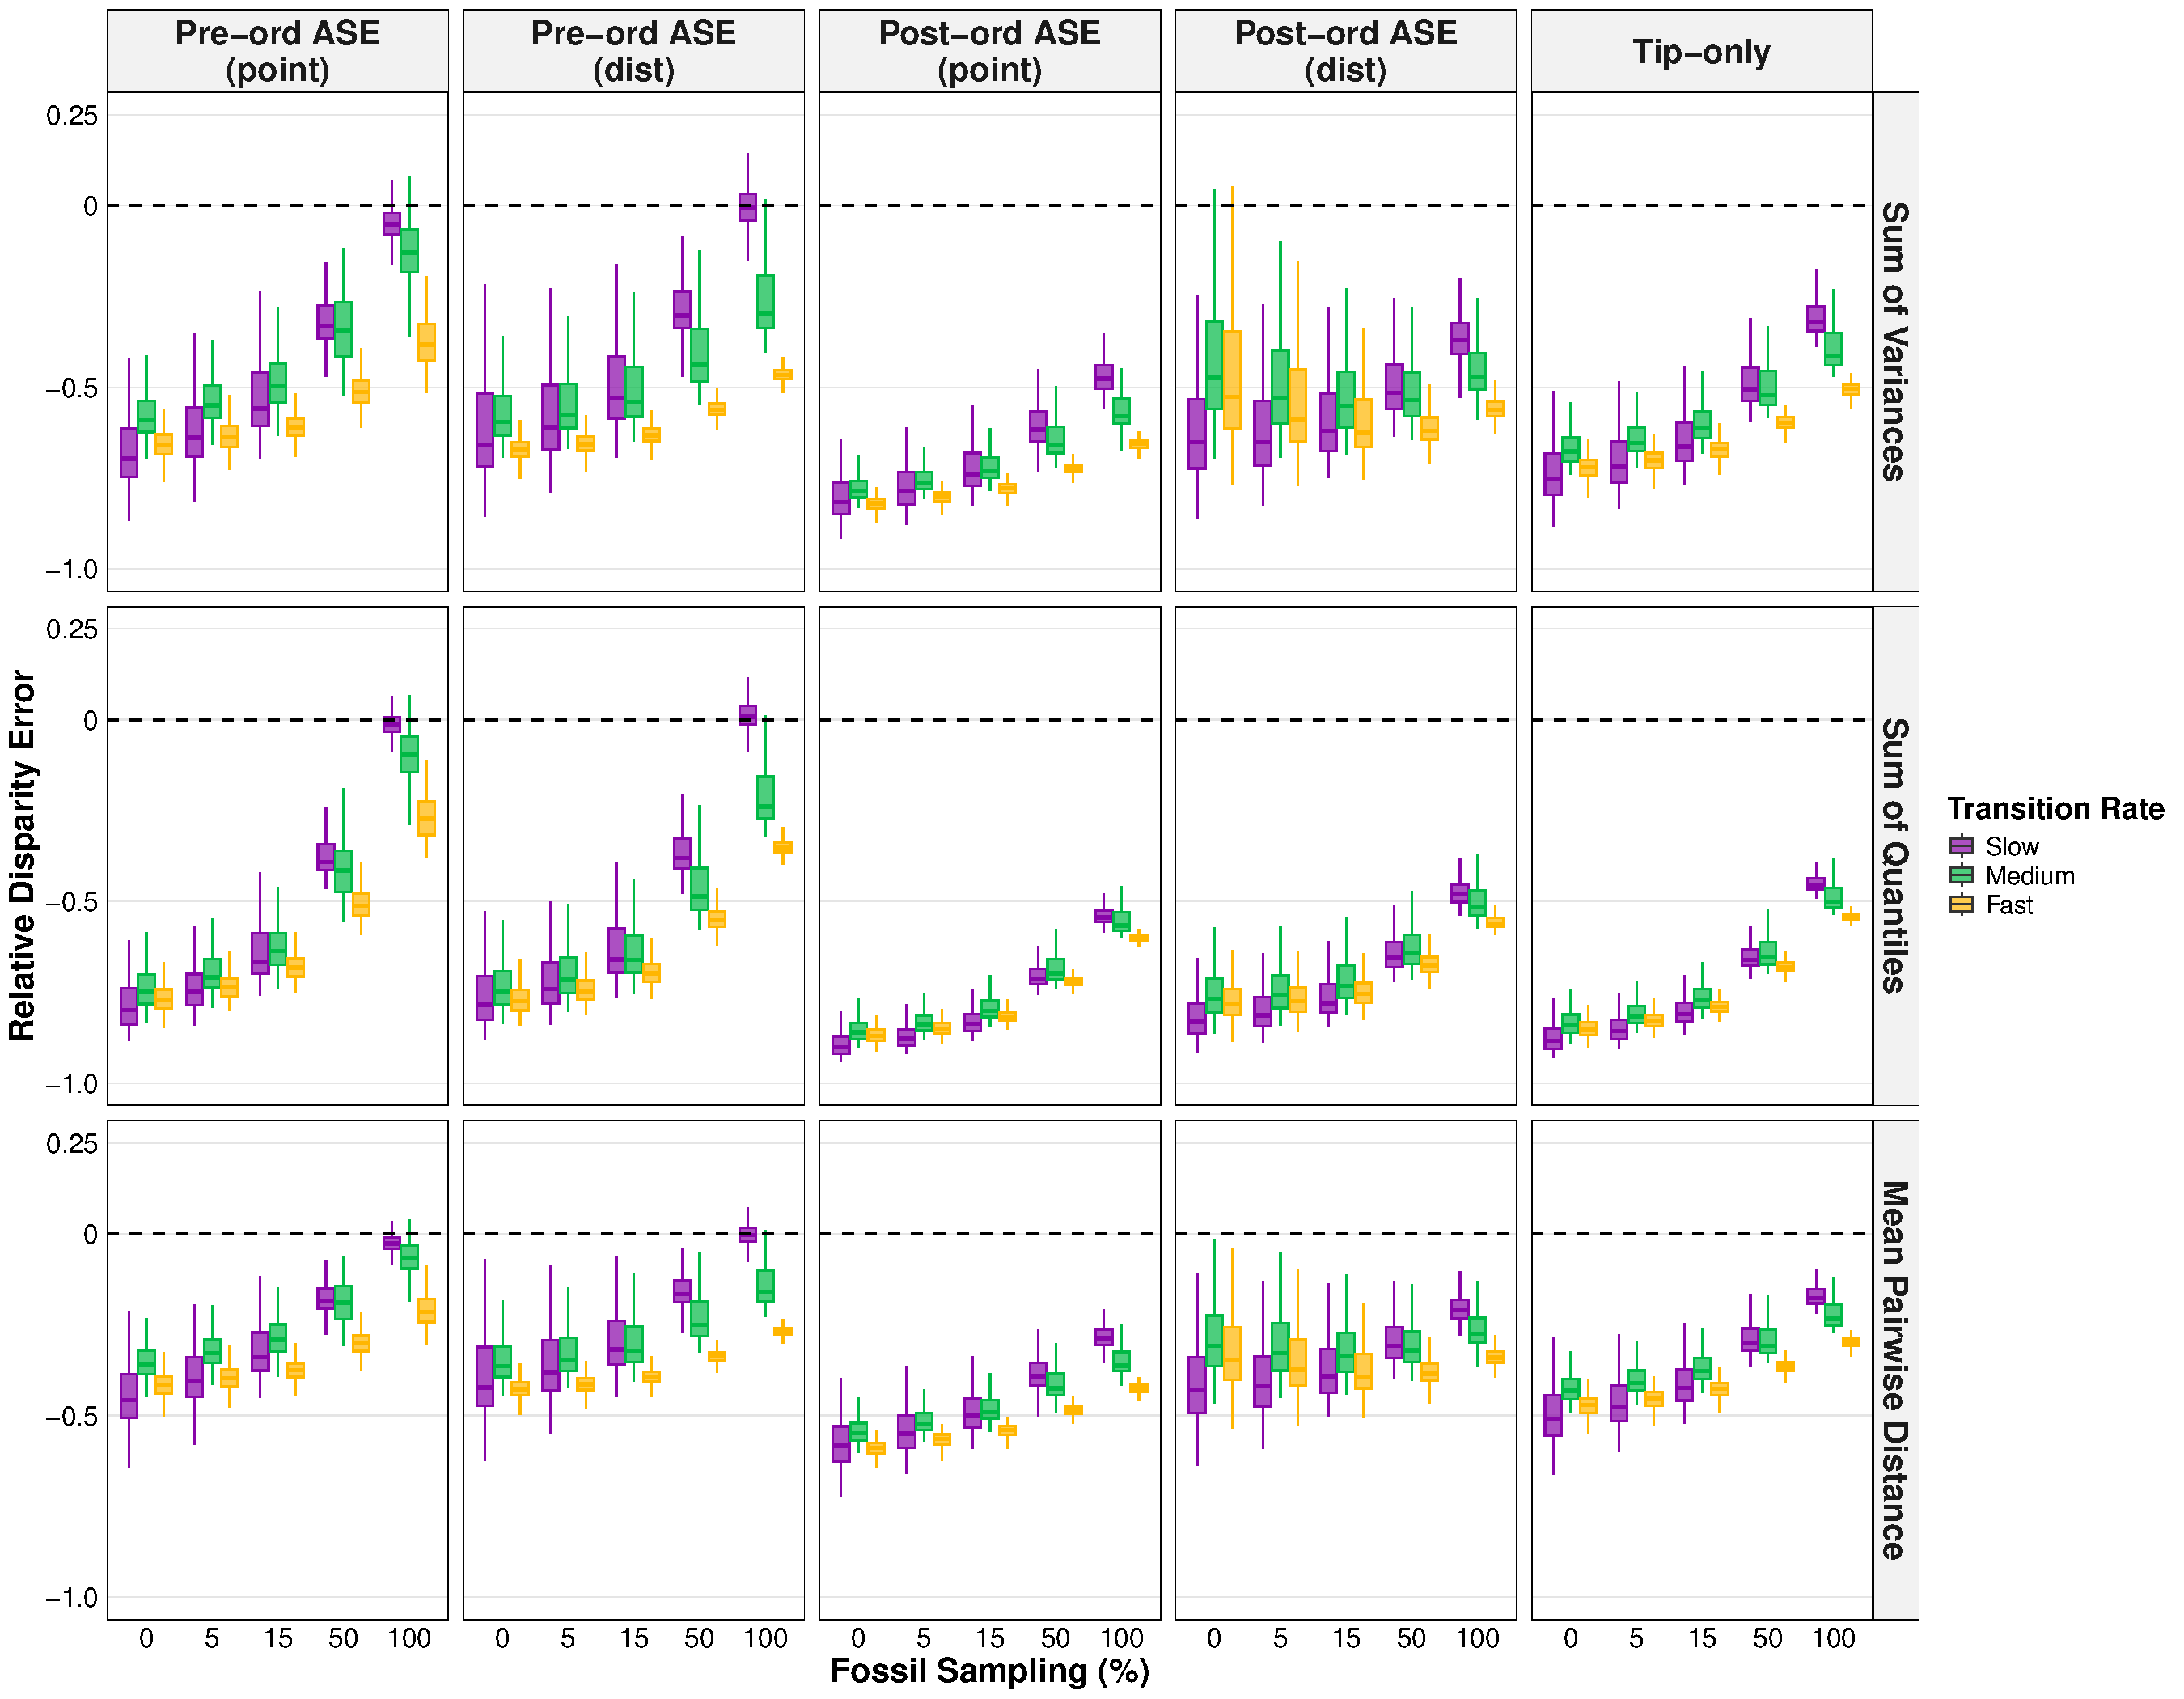
\includegraphics[width=1\textwidth]{figures/discrete_boxplot.pdf}
\caption{Relative disparity error returned from pre-ordination point ASE (ancestral state estimation), pre-ordination distribution ASE, post-ordination point ASE, post-ordination distribution ASE and no ASE. These disparity errors were calculated across three transition rates (fast (0.9), medium (0.1) and slow (0.01)), five simulated fossil sampling densities (100\%, 50\%, 15\%, 5\% and 0\%) and three disparity metrics (Sum of variances, sum of quantiles and mean pairwise distance). Values closest to 0 (dotted horizontal line) were most accurate; negative errors are under-estimates and positive are over-estimates.} 
\label{fig:discrete raw boxplot} 
\end{figure}


\subsubsection{Interaction effects} 
Similar to continuous traits, fossil sampling ($F_{4, 66976} = 22191, ~ p < .001$), transition rate ($F_{2,66976} = 6957,~  p < .001$) and metric ($F_{2,66976} = 26174, ~ p < .001$) were again major drivers of variation in accuracy.
As expected, increased fossil sampling and decreased transition rate led to lower disparity errors, and the mean pairwise distance was the easiest metric to recover, whereas the sum of quantiles was the hardest.
The three-way interaction between estimation method, fossil sampling and transition rate explained much of the variation in the data ($F_{32,66976} = 588, ~p < .001$; Table S4).
The broad pattern was that at high fossil sampling densities, pre-ordination point estimates were the best method, whereas at lower fossil sampling densities both pre- and post-ordination distributions returned the most accurate disparity values (\autoref{fig:discrete heatmap}).
This pattern was model-dependent, however, as under a slow rate the pre-ordination distribution method was the best performing method across all fossil sampling densities.
At fast and medium rates under low fossil sampling (< 15\%), the post-ordination distribution method returned the lowest disparity errors.
Notably, methods of ancestral state estimation outperformed their exclusion across all combinations of transition rate, fossil sampling density and disparity metric.
Again, while the disparity metric was a significant driver to overall accuracy, it had little effect on the hierarchy in methods set by the transition rate and fossil sampling density, signified by a weak four-way interaction ($F_{64,66976} = 10,~ p < .001$).

\begin{figure}[H]
\centering
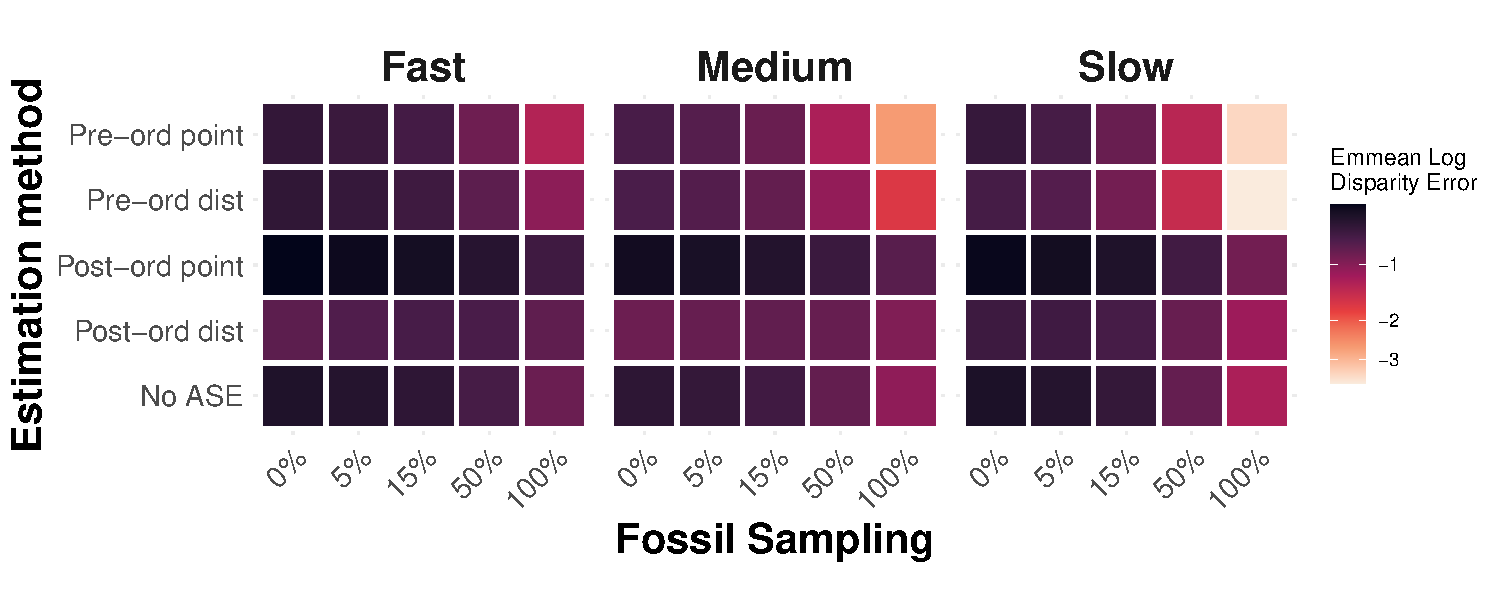
\includegraphics[width=1\textwidth]{figures/discrete_heatmap.pdf}
\caption{Heatmap showing the discrete estimated marginal mean (EMM) relative disparity errors for all combinations of estimation method, transition rate and simulated fossil sampling density. EMM were calculated from a linear mixed model with a three-way interaction, averaged across disparity metrics.} 
\label{fig:discrete heatmap} 
\end{figure}

\subsubsection{Sensitivity tests} 
Our findings did not differ under the alternative fossil sampling scheme (tips+nodes) %@@@add figure reference
or under asymmetrical trees (\autoref{fig:Asymmetrical trees boxplot}).
When we account for unequal dimensionality, we found virtually the same hierarchy of estimation methods as when we preserved the full dimensionality of the trait space (\autoref{fig:discrete fixed axes boxplot}), but note that the extent at which pre-ordination estimation methods were advantageous over excluding ancestral state estimations was slightly diminished.

\begin{figure}[H]
\centering
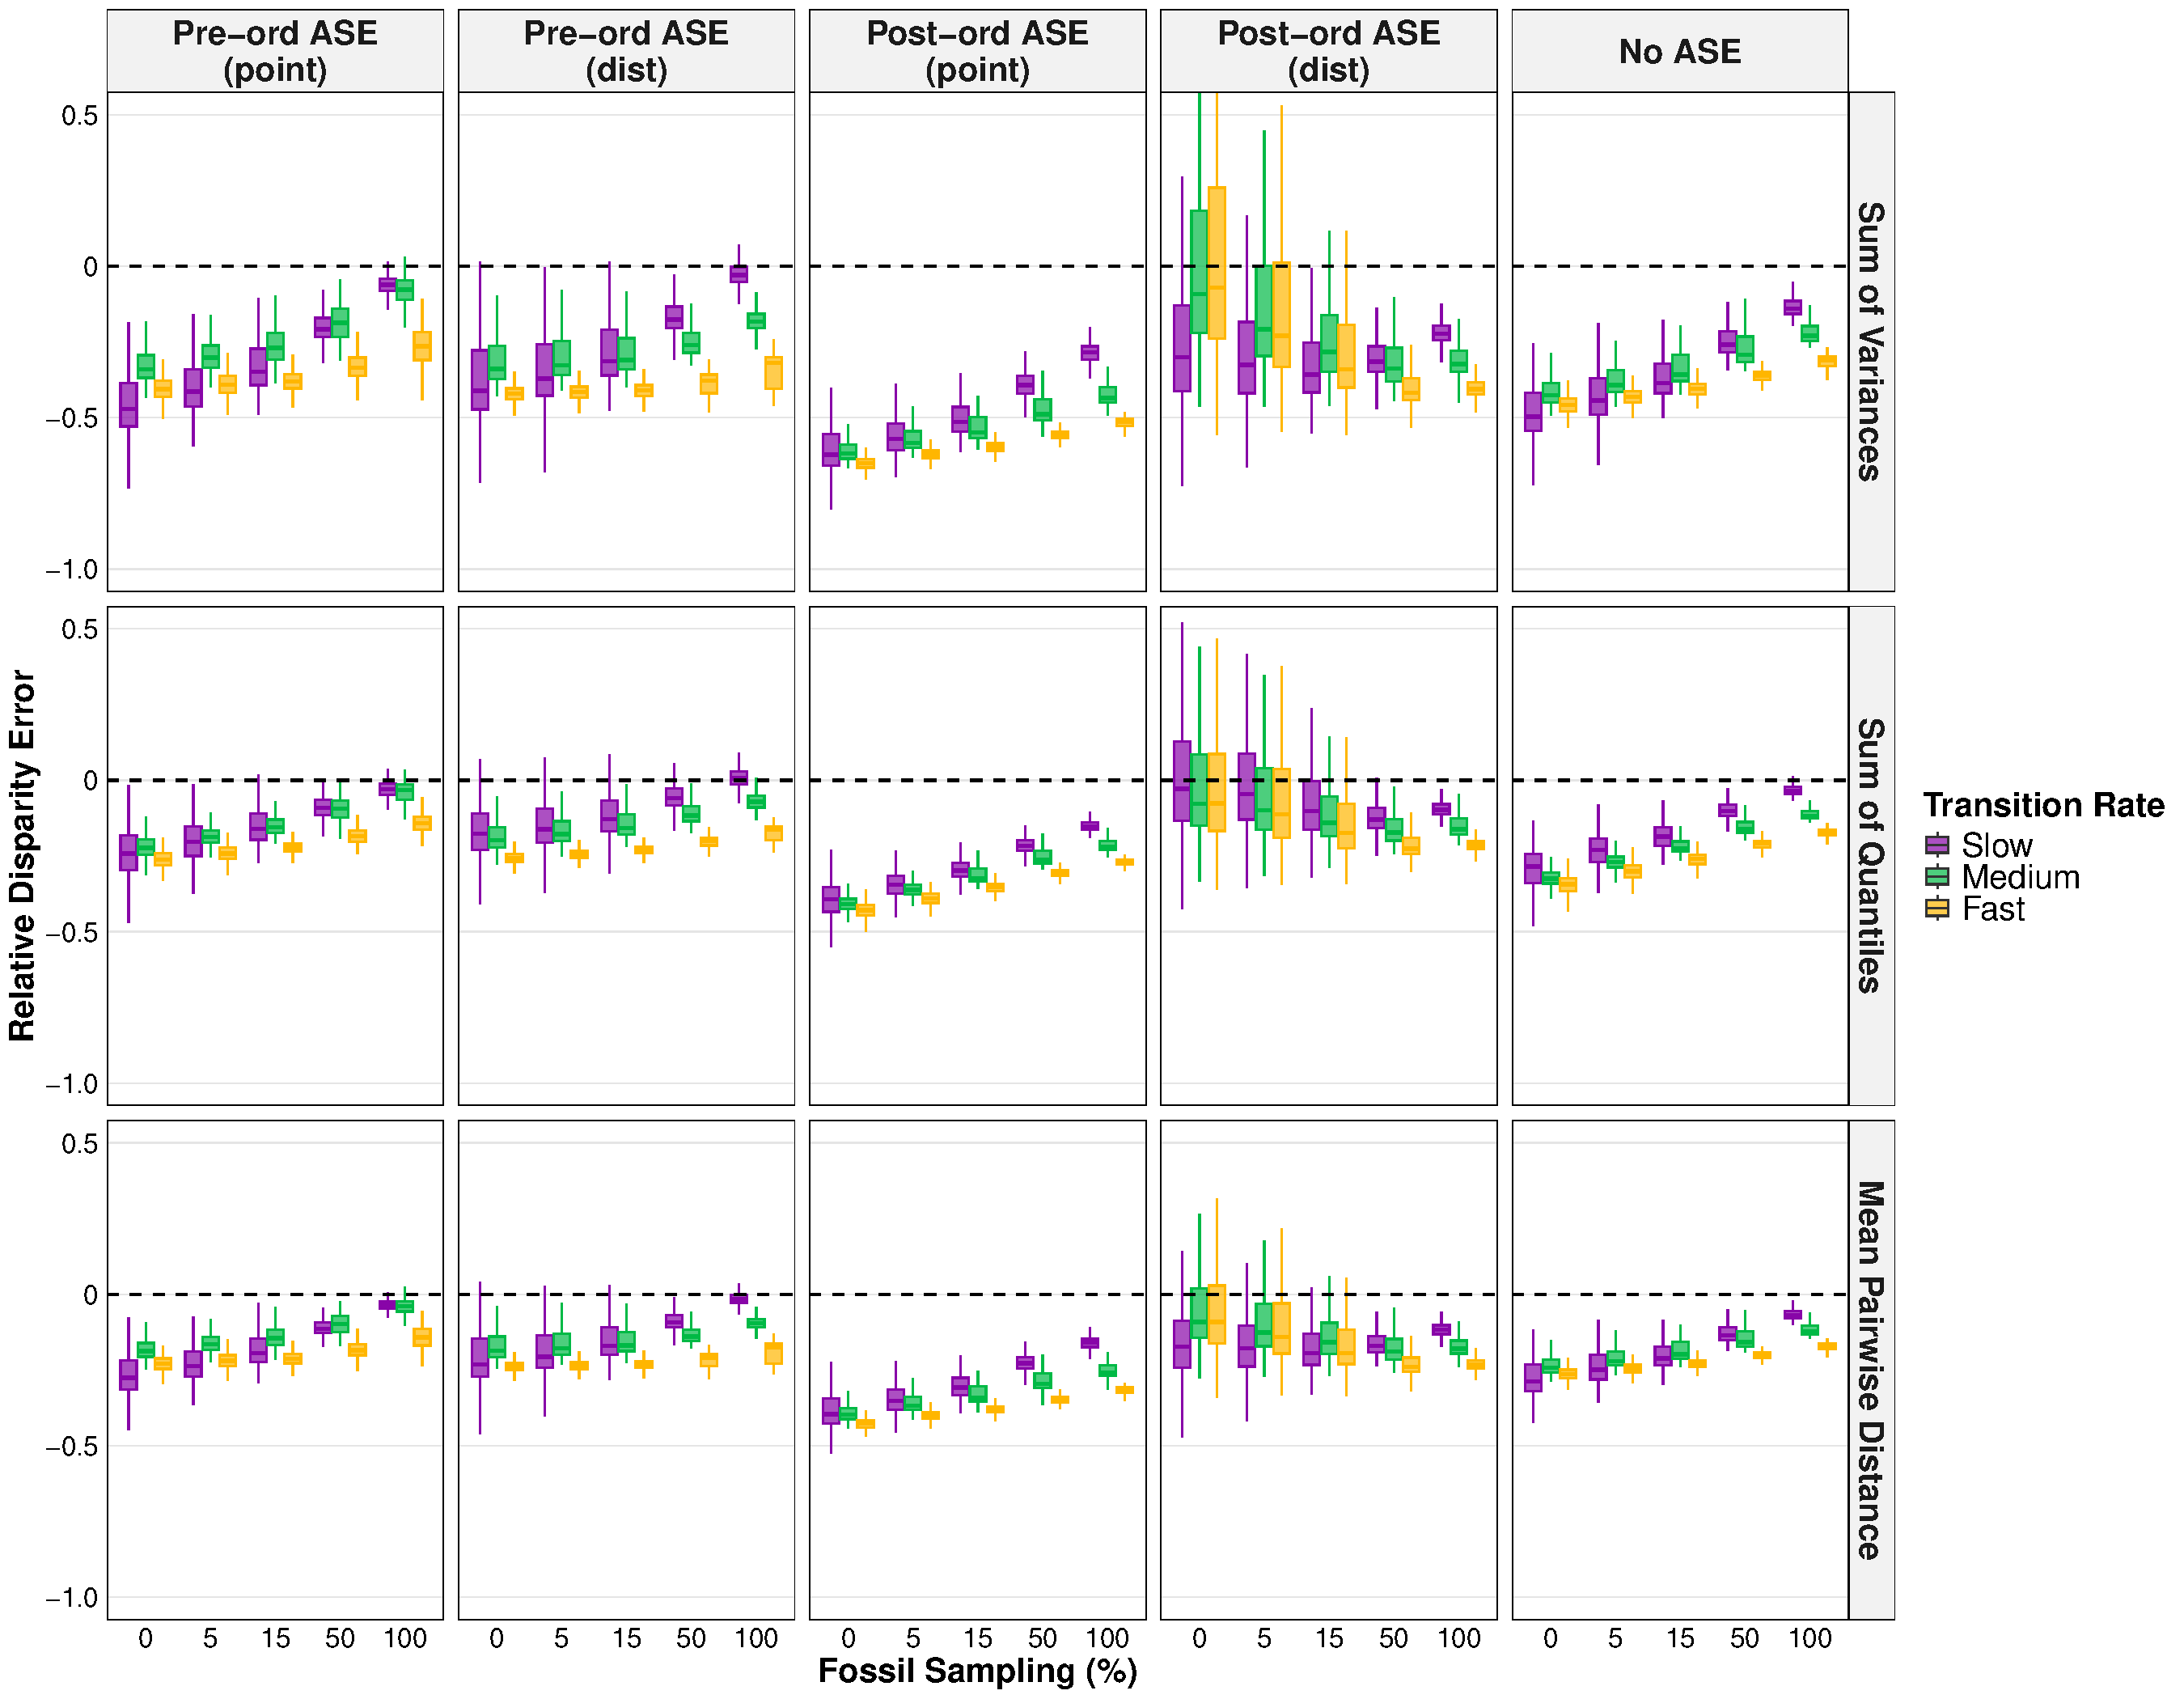
\includegraphics[width=1\textwidth]{figures/discrete_boxplot_rm_axes.pdf}
\caption{\textbf{fixed axes} Relative disparity error returned from pre-ordination point ASE (ancestral state estimation), pre-ordination distribution ASE, post-ordination point ASE, post-ordination distribution ASE and no ASE. These disparity errors were calculated across three transition rates (fast (0.9), medium (0.1) and slow (0.01)), five simulated fossil sampling densities (100\%, 50\%, 15\%, 5\% and 0\%) and three disparity metrics (Sum of variances, sum of quantiles and mean pairwise distance). Values closest to 0 (dotted horizontal line) were most accurate; negative errors are under-estimates and positive are over-estimates.} 
\label{fig:discrete fixed axes boxplot} 
\end{figure}

\section{Discussion}
Our results suggest that, generally, the inclusion of ancestral states improves the recovery of true disparity, defined here as the total region in trait space occupied by all members of a clade that have ever lived.
However, we found this to be context-specific, particularly dependent on fossil sampling and model of evolution.
Overall, we recommend that ancestral state estimations can consistently improve estimations of disparity derived from discrete characters, but recommend caution for continuous characters.

% \subsection{Continuous characters}
\subsection{Pre- versus post-ordination estimation}
For continuous characters, we found virtually no discrepancy between the effect of pre- and post-ordination estimation of ancestral states on disparity.
Given that continuous traits exist within a Euclidean space, the linear transformations of both PCA and \ase under Brownian motion (BM) mean that estimated node states exist within the same relative positions to the observed tip data for both pre- and post-ordination estimation. 
Note, however, that our simulated traits were uncorrelated.
In the case of non-orthogonality between traits, it is likely that the position of \ase in the disparity pipeline will have some effect, although this was not tested here.

For discrete traits, the position of \ase relative to ordination during the disparity pipeline (\autoref{fig:pipeline}) was a key driver in accurate recovery of the true disparity.
Overall, pre-ordination estimation led to more accurate disparity estimations than post-ordination estimation, a finding consistent with previous work  \citep{lloyd2018journeys}.
Post-ordination estimation is ultimately limited by the definition of the resulting trait space.
Axes of the trait space are treated as continuous traits evolving under BM, so, given the assumptions of BM, ancestral nodes are inevitably constrained within the bounds per-PC axis defined by the observed tip data \citep{stayton2015definition,lloyd2018journeys,gerber2019use}.
This forces the implicit assumption that our observed trait data accounts for the extremes of morphological diversity for the clade of interest, and that past diversity is only a subset of sampled diversity.
Disparity is therefore underestimated, particularly with range-based metrics such as sum of quantiles (\autoref{fig:discrete raw boxplot}).
Pre-ordination estimation does not encounter these same limitations.
A discrete trait matrix exists within a hypercube, where each vertex corresponds to a unique combination of traits.
When ancestral states are estimated prior to ordination, there is no constraint preventing an ancestor from occupying a legitimate and theoretically possible vertex that lies peripheral to the observed data \citep{gerber2019use}.
These ancestral nodes that lie outside the multidimensional convex hull defined by the tip data can inflate disparity relative to tip-only disparity \citep{brusatte2011phylogenetic}.
Similarly, authors have previously noted that inclusion of ancestral nodes can inflate disparity by (nearly) doubling the number of data points included in the trait space \citep{brusatte2011phylogenetic}, raising questions about whether such increases reflect genuine biological signal.
However, our findings demonstrate that the trait space expansion from the inclusion of ancestors, particularly when fossil sampling density is high, does converge on the true disparity of the clade under pre-ordination estimation.
% Furthermore, these concerns may be due to the choice of disparity metric (sum of quantiles) that is inhenrently less sensitive to sample size than other ones traditionally used (e.g. sum of ranges; \citealt{brusatte2011phylogenetic}). %TG: check if you agree with this or rephrase/delete. TL:DR; Brusatte's "raised questions" is just due to using inappropriate disparity metrics in that case.
As \autoref{fig:discrete raw boxplot} shows, underestimation of disparity is ubiquitous to all discrete character estimation methods, which has previously been linked to character exhaustion \citep{erwin_disparity_2007}.
Ultimately, pre-ordination discrete estimations are less susceptible to extreme underestimation because ancestral nodes are not bound to a weighted average of the tip data in the way post-ordination estimation is.

\subsection{Treatment of uncertainty}
The choice of estimation method for continuous characters was largely driven by the treatment of uncertainty.
At high fossil sampling densities, incorporating uncertainty through the use of distributions performed better than point estimates (\autoref{fig:continuous boxplot}; \autoref{fig:continuous heatmap}).
This is due to the tendency for point estimates to smooth over evolutionary history \citep{boyko2024dentist,boyko2026resolving}, underestimating the morphological variation of ancestral taxa.
However, in contrast to discrete traits, continuous estimation distributions are unbounded and thus sensitive to data quality.
Therefore, the variation introduced from sampling across a distribution was dependent on the density of fossils; at high fossil density, confidence intervals are constrained due to lower uncertainty in estimates. %TG: changed to uncertainty for consistency
As fossil sampling decreases, these confidence intervals are widened and more noise is introduced as a result of using distribution \citep{schluter1997likelihood, martins1999estimation}, negating the advantage observed at higher fossil sampling.

For discrete characters, we found an inverse pattern where distribution methods were optimal at low fossil sampling densities and point estimates were optimal at high fossil sampling densities.
This is likely due to the bounded nature of discrete traits; even with minimal information, the disparity error that can be returned is bounded by the number of states present at each node, which contrasts the effectively infinite error that can be returned by continuous characters.
Regarding pre-ordination estimations, our results reveal two issues relating to uncertainty.
At low fossil sampling or slow transition rates, the predominant issue facing the recovery of a true trait space is the lack of data.
For fossil sampling, the lack of evidence in deeper time means our ancestral state estimates, and subsequent trait space pattern, are biased by the living tip data. 
In the case of slow transition rates, we face a paradoxical situation with slow rates where the root state can be easily estimated, yet the few transitions make the rate of change hard to estimate \citep{gascuel2020darwinian}.
Using the hypercube analogy again, the state scaled likelihoods at each node under slow rates or low/absent fossils will be biased against transitions.
Therefore, because point estimations essentially recover the most parsimonious evolutionary history, ancestral nodes will be constrained within a certain region of vertices in the trait space.
In contrast, pre-ordination distribution estimations allow the exploration of other vertices by sampling across alternative discrete state combinations.
In the case of slow rates and low fossil sampling, this was found to improve disparity estimations (\autoref{fig:discrete heatmap}).
The flip side of this is the issue of saturated data, where the paradox is reversed and instead, we have an abundance of information, thus transition rates are easy to estimate, yet due to the rate of change most nodes are left with inconclusive scaled likelihoods.
Under the fast rates simulated in this study, character transitions are saturated, so there is very little phylogenetic signal.
The use of distributions amplifies the noise in this scenario, thus point estimates can be used to filter out the noise which is why they outperform distributions at medium/fast rates (\autoref{fig:discrete heatmap}). 




\subsection{Model misspecification and fossil inclusion}
As expected, we found that the differences in true and simulated disparity across models of evolution reflect model misspecification in ancestral state estimation.
The inclusion of ancestral state estimations recovered a more accurate trait space than excluding ancestral states across all fossil sampling densities and disparity metrics when Brownian motion was the evolutionary model.
Ancestral state estimation of continuous characters uses the BM model as an assumption for the evolution of traits, so this was expected.
The assumptions of BM include a fixed mean and trait variance increasing linearly through time \citep{felsenstein1985phylogenies,omeara2006testing}.
We found that when these assumptions of BM were violated, such as under BM + trend and OU models, disparity accuracy returned by methods with \ase decreased.
For example, under low/absent fossil sampling, methods of \ase performed worse than bypassing ancestral state estimation for BM + trend.
In this case, disparity estimates tended to be underestimated, because state estimations will be intermediates of the observed tip data, absent to the directional trend that occurred and thus missing drifted regions within trait space.
Our results suggest a threshold between 5-15\% fossil sampling where \ase becomes optimal over its exclusion in disparity (\autoref{fig:continuous heatmap}).
This finding supports previous work that highlights the critical impact of fossil inclusion when directional trends are present in the trait data \citep{finarelli2006ancestral,albert2009fossils,slater2012integrating,finarelli2013potential,gearty2024impact}.

Similarly, calculations of disparity derived from OU simulations were also underestimated when using ancestral state estimations.
The OU process is characterised by a stationary variance, which contrasts the BM assumption of an increase in variance through time.
Therefore, because BM estimates internal nodes as a weighted average of the observed tip data, the ancestral nodes are compressed towards the centroid of the trait space. 
This explains why, when model misspecification is fundamentally incorrect, bypassing \ase outperforms the use of ancestral state estimation, even with 100\% fossil sampling. 
We therefore encourage model-fitting prior to performing \ase to avoid model misspecification; several \texttt{R} packages allow model-fitting and estimation of continuous traits under an OU model \citep{revell2012phytools,pennell2014geiger,clavel2015mvmorph}.
Note that empirical studies of disparity tend to focus on clades that are suspected to have undergone major evolutionary shifts, such as adaptive radiations \citep{ruta2013decoupling,stroud2016ecological} or mass extinctions \citep{bapst2012graptoloid,halliday2016eutherian,liu2024heterogeneous}, which are often associated with shifts in evolutionary rates or models. 
The effect of such shifts or heterogeneity in the context of the aims of this paper remains to be tested; previous work has found that rate changes are hard to detect and can lead to erroneous inferences in single-trait ancestral state estimations (\citealp{king2015ancestral,chira2016impact, harrington2017rate}; but see \citealp{reyes2018testing, muniz2025robustness}).
Several recent methodological developments have aimed to accommodate for rate heterogeneity in both continuous \citep{elliot2014inferring,smaers2016multiple, castiglione2020ancestral} and discrete ancestral state estimation \citep{boyko2021generalized,revell2024discrete} and so the testing of these methods in the context of disparity is a potential future avenue of research.



%% need something on fossils and where we are actually at empirically with fossils.


% However, in the case of the OU-derived disparity, disparity values returned from \ase were not necessarily far off those that bypassed ancestral state estimation, so the decision whether to use \ase in this scenario is a trade-off between the slight decreased accuracy of estimations versus the advantages of incorporating ancestral states in disparity analyses. 
% therefore, fitting correct model of \ase would fix this?

% however, even though bypassing \ase is better in this scenario with OU, the use of distribution estimations is still relatively well performing with a low relative disparity error. Therefore, it is a tradeoff of the benefits that come with using ancestral states (able to look further in deep time etc) vs absolute disparity accuracy.

% - discrete ancestral state estimation is always more accurate than non ancestral state estimation.
% - it would be interesting to test if discrete trait estimation follows same issue with recovering trait space if there is rate heterogeinity, or unequal transition rates (violation of ER).
% - However, several studies have found that raw accuracy of recovering true state can be robust against model misspecification (i.e. ARD vs ER) and rate heterogeneity.




\subsection{Simulation sensitivity tests \& limitations}

% 1.
%     a) asymmetry did not change results, we actually found an improvement
%     b) link to keating's paper
% 2. Generally, results did not change between fossil sampling approach
%     a) tips-only is the conventional approach, given that when we sample a fossil we do not know whether it is represents a node or fossil
%     b) we incorporated the nodes as a way for testing whether that biases our findings:
%         (i) for discrete traits, we found no difference. this is because under discrete simulation, a tip and node are morphologically diverse as each other
%         (ii) continuous traits, we did find this sampling method changed results, because ancestors are by definition less variant etc (recycle response to wagner)
%     c) our results assume the bifurcating model of phylogeny as the evolutionary history, but acknoweldge that other mechanisms of speciation, such as budding or anagenesis, could affect the results. we acknowledge the simplicity in the fossil sampling scheme.
% 3. Dimensionality
%     a) whether the dimensionality is an attribute of a 'true disparity value' is up for debate.#


Simulations are increasingly used across computational evolutionary biology to evaluate methodological approaches \citep{lotterhos2022simulation}.
However, given the complexity of morphological evolution across clades, generalising simulation procedures is an endeavour that offsets empirical and biological realism \citep{goloboff2018parsimony,o2018empirical}.
Our simulation procedures have focused on empirical realism to replicating the workflow that authors that use ancestral states and disparity estimations undergo.
However, we acknowledge that this is at the expense of some biological realism.
To account for these, we ran several sensitivity tests.
For example, we tested for the effect of asymmetry on our results (\autoref{fig:Asymmetrical trees boxplot}) and found congruent patterns in estimation hierarchy across treatments to our main findings. 
Raw ancestral state estimation accuracy has been shown to increase as tree asymmetry increases, since asymmetrical trees have fewer nested internal nodes, albeit the increased branch lengths can increase uncertainty in estimations \citep{keating2023best}.
We observed this exact pattern, with the generally lower disparity error across asymmetry trees, albeit with wider error within pre-ordination estimation methods.

% Similarly, we also tested whether our tip-only fossil sampling scheme was influencing our results, by implementing an alternative scheme that allowed nodes as well as tips to be sampled as fossils.
While we found no influence in fossil sampling scheme on our discrete trait results, we found that the BM model results in continuous traits were influenced by the fossil sampling scheme; specifically that the sum of quantiles recovered by \ase methods was an underestimation compared to bypassing ancestral state estimation.
This finding is indicative that restricting our sampling scheme to tips, which by definition will be the most morphologically distinct taxa under BM since they are the furthest patristic distance from the root, will inflate our disparity estimates.
Naturally, we are not able to identify fossils as nodes or tips at the point of discovery, which is why our main findings use the fossil sampling scheme that represents empirical realism.
However, we acknowledge that this is at the expense of biological realism.

Dimensionality was also shown to have an effect on disparity error.

There are still several assumptions/factors that we have not accounted for, that can influence both ancestral state estimaton and disparity analyses. 
Firstly, is phylogenetic uncertainty.
Secondly, is fossil preservation level; while we focus here on the lineage sampling, we assume perfect fossil preservation. 
We advise that the Pre-OASE1 method of ancestral state estimation is implemented, so that only characters that have observed tip data descending from that node are estimated.



% it could be said that our original fossil sampling scheme of only sampling fossils, represents the actual bias we find in our fossil sampling. When we sample a fossil, it is more likely to be a tip (on a new branch) wheres nodes are less likely to be sampled due to cryptic species. So, our tip-only analysis in some ways represents empirical realism


% however we note that the magnitude of error is small compared to other contrasts mentioned in the study.





% \subsection{Disparity metrics and recovering a true trait space}
% % 1. Generally, the disparity metric did not change the hierarchy of methods
% %     (a) Some methods were easier to estimate than others
% %     (b) Sum of quantiles
% %         (i) Distribution methods were best performing here
% %         (ii) For discrete characters, it is essential to use pre-ordination distribution if using a range based metric, because post-ordination will constrain your range within the sample of tip data, and point estimates do not allow the expansion of variance that is needed.
% %     (c) Sum of variances / mean pairwise dist
% %         (i) Behaved very similarly
% %         (ii) Generally harder to estimate in continuous characters 


% %The mercy of continuous traits
% %         (i) Near misses (i.e. guessing a trait value to be 11 when in truth it was 10) is more graceful on traitspace than getting a discrete state wrong?
% %         (ii) Although comparing discrete vs continuous estimation of disparity not a main question in this study, it would be interesting


% Previously, the choice of disparity metric has been probed as a critical step in the disparity pipeline, specifically for examining different aspects of trait space \citep{guillerme2020shifting, guillerme2025and}.
% Indeed, our results exhibit significant differences in disparity error among metrics.
% For example, recovering the sum of quantiles was ultimately harder than recovering the sum of variances or mean pairwise distance when using discrete traits.
% However, the hierarchy of methods was relatively consistent across disparity metrics, suggesting that the relative performance of ancestral state estimation methods is robust to different disparity metrics.
% Consistent performance across multiple disparity metrics can reassure us that multiple aspects of the true trait space are recoverable, such as size and density.
% Where there is inconsistency in methods across metrics, we can infer that the true disparity value has been attained as a methodological artefact, rather than the recovery of a true trait space pattern. 
% This can be observed in the post-ordination distribution estimation of discrete traits, which performed well under the sum of variances and mean pairwise distance metrics, but noticeably worse under sum of quantiles.
% From this we can infer that while the internal density of taxa was correctly recovered, the geometric constraint of post-ordination estimation ultimately limited its ability to recover true trait space expansion.
% % This was a ubiquitous problem across methods, indicating that, without the impossible achievement of a complete fossil dataset, our calculations of the absolute size of trait spaces will always be an underestimation. 

\subsection{Conclusions and recommendations}
Our findings present a convincing case for the use of ancestral state estimation in disparity analyses, a method that has often been neglected in disparity workflows.
Furthermore, our results issue a stark reminder of the essential need for fossils during macroevolutionary workflows.
The estimated proportion of fossils sampled across empirical datasets is typically less than 5\% \citep{raup1976species}, which ultimately limits our inferences into macroevolutionary patterns.
However, in the case of discrete traits, the incorporation of ancestral states is more optimal than their exclusion across all fossil sampling densities, and the same is true of continuous traits when the correct model is used for estimation.
Based on these findings, we can recommend the following guidelines for the use of ancestral state estimation in disparity analyses: 1) for continuous traits, perform model testing prior to running ancestral state estimation to infer the likely evolutionary model parameters, and then estimate ancestral states under this model, using the distributions of estimates in disparity analyses; 2) for fast/medium rate discrete traits, pre-ordination point estimates should be used when fossil sampling is suspected to be less than 15\% and post-ordination distribution when fossil sampling is lower than this. Pre-ordination distribution should be used when transition rates are slow across all fossil sampling densities. 




% Below we have written a TL;DR

% Based on these findings, we can recommend the following guidelines for the use of ancestral state estimation in disparity analyses:
% \begin{enumerate}
%     \item For continuous traits, use distributions of estimations, rather than point estimates. If the trait data is suspected to have evolved under OU model, estimation of ancestral states assuming an OU model is critical.
%     \item For discrete traits, pre-ordination point estimations are optimal when transition rates are
% \end{enumerate}

% \textbf{Key takeaways (continuous):}
% \begin{itemize}
%     \item Use \textbf{distribution} estimations when trait data fits a BM (or BM + trend) model of evolution.
%     \item If trait data is best fitted by a BM + trend model, fossil sampling >5\% is essential to return a reliable disparity signal.
%     \item If trait data is best fitted by an OU model, ancestral states should be excluded at all fossil sampling densities (but still relatively accurate using ancestral states).
% \end{itemize}



% \textbf{Key takeaways (discrete):}
% \begin{itemize}
%     \item Use \textbf{pre-ordination point} estimations when fossil sampling is dense >15\% and transition rates are medium/fast
%     \item Use \textbf{post-ordination distribution} when fossil sampling is low <15\% and transition rates are medium/fast
%     \item If rates are slow, the \textbf{pre-ordination distribution} method is best across all fossil sampling densities
%     \item It is encouraged to always use \ase, because it improved estimations of disparity across all scenarios.
% \end{itemize}







% why continuous > discrete -> continuous traits preserve larger variation in state space \citep{parins2018use}

% 3. Other considerations: 
%     a) How this translates to disparity through time
%       (i) most clades that are studied are usually studied because they do something interesting, or it is across a mass extinction etc. Therefore, in these instances, we would expect some level of rate heterogeinity, or model switch etc. Therefore, we highlight that fossils and model-testing is essential prior to estimation, as well as the use of distribution methods (particularly since)
%     b) Different methods of ancestral state estimation
%         (i) other there are other methods of ace (some of which have been shown to perform better than Mk model used here), then we could expect estimations of disparity to improve.
%         (i) Main consideration is that generally using a distribution is best.
%     c) Rate heterogeneity was not considered, but we expect for disparity that it would not change results much -> it seems for disparity, raw accuracy of states does not have a cascading effect on innacacy of disparity as much as the actual absence of points in trait space.
%     d) subclade disparity etc, how well partitioned in trait space subclades are to the ground-truth.



% being able to estimate the transition rate may be enough for disparity, rather than exact states? i.e. in a situation of fast rates, where say none of the states are estimated correctly, but disparity signal is accurate, because a similar dispersion of trait space has been reached.

% Second, use of discrete characters may create a problem with character exhaustion and could produce underestimates of disparity relative to studies using continuous characters  (Erwin 2007)




\section*{Acknowledgments}

CNS would like to thank Robin Beck, Russell Garwood and Vera Weisbecker for thoughtful discussions about the study. TG acknowledges funding from NERC-UKRI Grant NE/X016781/1. Thank Stanage...

\section*{Author Contributions}

\textbf{Conceptualisation} CN Scutt (CNS), GH Thomas (GHT), N Cooper (NC), T Guillerme (TG); \textbf{Data curation} CNS; \textbf{Formal analysis} CNS; \textbf{Funding acquisition} TG; \textbf{Investigation} CNS, TG; \textbf{Methodology} CNS, TG; \textbf{Project administration} CNS, GHT, NC, TG; \textbf{Resources} CNS, TG; \textbf{Software} CNS, TG; \textbf{Supervision} GHT, NC, TG; \textbf{Validation} CNS; \textbf{Visualisaton} CNS; \textbf{Writing - original draft} CNS; \textbf{Writing - review \& editing} CNS, GHT, NC, TG.

\section*{Data Availability}

The code to reproduce the analyses is available here \url{https://github.com/calebowski/acedisparity} \citep{caleb_scutt_2026_19665049}.
Data is available at \url{https://doi.org/10.5061/dryad.280gb5n4p}.

\section*{Competing Interests}

We declare no conflict of interest.


\clearpage

\bibliographystyle{plainnat}
\bibliography{references.bib}

% \printbibliography

\end{document}